\documentclass[sigconf,authorversion,nonacm]{acmart}

\AtBeginDocument{%
  \providecommand\BibTeX{{%
    \normalfont B\kern-0.5em{\scshape i\kern-0.25em b}\kern-0.8em\TeX}}}
\usepackage{hyperref}

\begin{document}

\settopmatter{printacmref=false}

\title{Internet weather maps and statistics: Which ones exist?}

\author{Bashar Khoulani}
\email{bashar@uni-kassel.de}
\affiliation{
  \institution{Universität Kassel - Distributed Systems}
  \city{Kassel}
  \state{Hessen}
  \country{Germany}
}

\begin{abstract}
The use of Internet weather maps and statistics has become increasingly important for institutions, as it provides valuable insights about their networks, applications, benefits, and limitations. These statistics can include information such as the bandwidth between two devices, packet frame sizes, or temporal events, which can help organizations detect congestion and anomalies and analyze recurring events. 

In this paper, I will delve deeper into the background of Internet weather maps and statistics, discussing their advantages and disadvantages. As the main focus, I will refer to the Internet weather maps that currently exist. By understanding the usefulness of Internet weather maps and statistics, organizations can make more informed decisions about network management, troubleshooting, and overall optimization.
\end{abstract}
\maketitle
\section{Introduction}
In data networking, the concept of Internet weather refers to the varying conditions of network performance, much like meteorological weather reflects atmospheric conditions. Network weather is gauged through several key performance metrics such as availability, latency, load, and packet loss. These metrics serve as indicators of the network's health, similar to how temperature, wind speed, and pressure are used in weather forecasting.

The collection of network performance data is typically done through two methods: active and passive. Active measurement involves the process of sending test packets through the network to monitor their progress, whereas passive measurement relies on observing traffic flow at specific points. This difference is similar to using rain gauges and Doppler radar in meteorology.

An interesting development in this field is the creation of Internet weather maps. These maps provide visual summaries of network performance, displaying information like traffic flow through color-coded links. They offer a simplified, user-friendly interface for both network customers and the public, helping identify network issues and providing access to more detailed statistics. However, the information presented is often limited due to security and confidentiality concerns and is typically aimed at providing a general overview rather than detailed technical data. 

The metrics that are used in network weather maps include the availability of the network, which refers to the percentage of time that the network is available to users. The latency of the network is another metric, which measures the time it takes for data to travel from one point to another on the network. The load of the network is the amount of data that is being transmitted through the network at a given time. Finally, packet loss is a measure of the number of data packets that are lost or not delivered to their intended destination.

Active measurement techniques are usually performed by sending test packets from a source to a destination and then measuring the time it takes for those packets to travel that distance. This is typically done by sending a ping request to a device on the network and measuring the response time. Passive measurement techniques, on the other hand, involve the collection of data from network devices that are already in use. This is done by observing the traffic flow at specific points in the network, such as routers or switches.

An internet weather map is, therefore, a tool that provides a visual representation of a network's structure and its connections between devices. It includes bandwidth measurements that help identify potential issues and anomalies that the network might experience. By monitoring the network through the weather map, network administrators can detect any unusual events and investigate the cause of the problem. 

To gain further insights into the network's performance, statistics are collected and analyzed over regular intervals. The statistics provide information about the usage of network nodes and routers, including peak events and possible anomalies. The aggregated statistics can help identify recurring trends and issues that might affect the network's overall performance. By analyzing the statistics, network administrators can proactively address any potential problems and ensure the network is running efficiently.

In the following section, some of the most common network issues will be mentioned and explained. 
\subsection{BACKGROUND}
\textbf{Congestion:} Network congestion is a widespread issue that can significantly reduce the quality and performance of a network. This problem usually occurs due to a network node that processes data beyond its capabilities. Congestion is often caused by insufficient bandwidth, poor network design, or node failures, which result in delays in processing packets, eventual packet loss, and a general decline in network performance \cite{simulation}.

To address this problem, various methods have been developed to mitigate network congestion. One of the most commonly used methods is Random Early Detection (RED), which monitors the queue of the network node and discards packets before the queue becomes full. Another method is flow monitoring, which monitors the flow of data in the network and identifies congested areas. Moreover, there are several protocols and algorithms embedded in switches and routers that help in preventing network congestion. These protocols and algorithms include traffic shaping, Quality of Service (QoS), and Multiprotocol Label Switching (MPLS), among others.

Network congestion is a complex issue requiring careful monitoring and management to ensure optimal network performance. Understanding the causes and implementing effective methods to mitigate this problem is crucial for maintaining a reliable and efficient network.

\textbf{Anomalies:} Networks are complex systems that require constant monitoring to ensure seamless functioning. However, in large networks, certain elements can cause irregular traffic patterns, which deviate from the normal behavior of the network. These elements are known as anomalies and can affect the network's performance. It is crucial to detect anomalies as they could be an indication of a potential security breach or a change in network dynamics.

By analyzing weather maps and statistics, information about the anomalies' sources, dates, and times can be collected. This information can help identify the root cause of the anomalies and provide a conclusive explanation behind them. For instance, sudden traffic spikes at odd hours may indicate a potential security breach, while gradual changes could indicate changing user behaviors or changes in network dynamics.

It is important to note that some anomalies can be malicious and caused by bot attacks \cite{6524462}. Therefore, detecting and addressing these anomalies is essential to ensure network security and maintain optimal network performance.

\section{Motivation and Ethics}
Many institutions deploy monitoring software on their networks to protect the infrastructure. The monitoring software and its output come close to Internet weather maps and statistics. On a global level, they introduce bigger benefits which could be several of the following:

\textbf{Intrusion and anomaly detection:} The vast network of the internet generates an enormous amount of data, which is constantly being collected and analyzed to identify patterns and trends that deviate from the norm. Internet weather maps and statistics play a crucial role in providing a comprehensive view of network performance and traffic. 

For instance, sudden spikes in traffic could indicate a bot attack on the network, while an increase in latency or packet loss could suggest a network congestion issue. To detect such anomalies, CDNs (Content Delivery Networks) rely on advanced techniques of graph theory and artificial intelligence.  CDNs can leverage these advanced techniques to model the network and detect any deviation from the normal traffic pattern. This enables them to identify and mitigate the impact of network attacks, such as DDoS (Distributed Denial of Service) attacks, before they cause any significant damage. Furthermore, CDNs can enhance network security by improving intrusion detection capabilities and anomaly detection techniques. By analyzing the network traffic in real time and comparing it to historical data, CDNs can identify suspicious activities and take proactive measures to prevent security breaches. 

\textbf{User experience:} In today's world, network providers have access to a vast amount of data about users' online behavior, which can be leveraged to make informed decisions and tailor content. By analyzing Internet weather maps and collecting large datasets about interactions and time spent on selected websites, providers can gain valuable insights into usage patterns and trends. For example, they can identify how users' internet usage changes during different seasons, such as winter or spring, and use this information to optimize resource allocation or enhance overall user satisfaction. This data-driven approach can also help providers offer personalized content and services that meet the specific needs and preferences of individual users.

\textbf{Network management:} Internet weather maps and statistics are important tools for analyzing the performance of a network and maintaining its functionality. These tools help identify potential bottlenecks and network requirements that can be addressed promptly, such as predicting capacity bottlenecks and hardware failures. By analyzing internet weather maps and statistics, you can gain insights into network performance and use network resources efficiently, optimizing the user experience. This is particularly important for content delivery networks (CDNs), where timely content delivery is critical for business success. In essence, internet weather maps and statistics help businesses stay ahead of potential network issues and proactively take steps to maintain their networks, ensuring that customers receive the best possible experience when accessing their content.

\textbf{Users' privacy:} One potential drawback of utilizing weather maps and statistics is the potential risk it poses to the privacy of users, particularly about their payload, IP, and MAC addresses. This risk is magnified if the collected datasets are intended to be used for research purposes. To address this issue, the datasets must be carefully cleaned and anonymized. Specifically, any payload data must be removed and the addresses must be scrambled in such a way that users cannot be identified. Achieving this requires significant manpower and resources to carry out the anonymization process effectively \cite{271335}.

Overall, Internet weather maps and statistics mark a new era in network administration. They transform raw data into insightful information that leads to informed, smart, and knowledgeable actions.

\section{Related works}
This section will refer to several existing Internet weather maps and statistics and their research contributions.
\begin{figure}
    \centering
    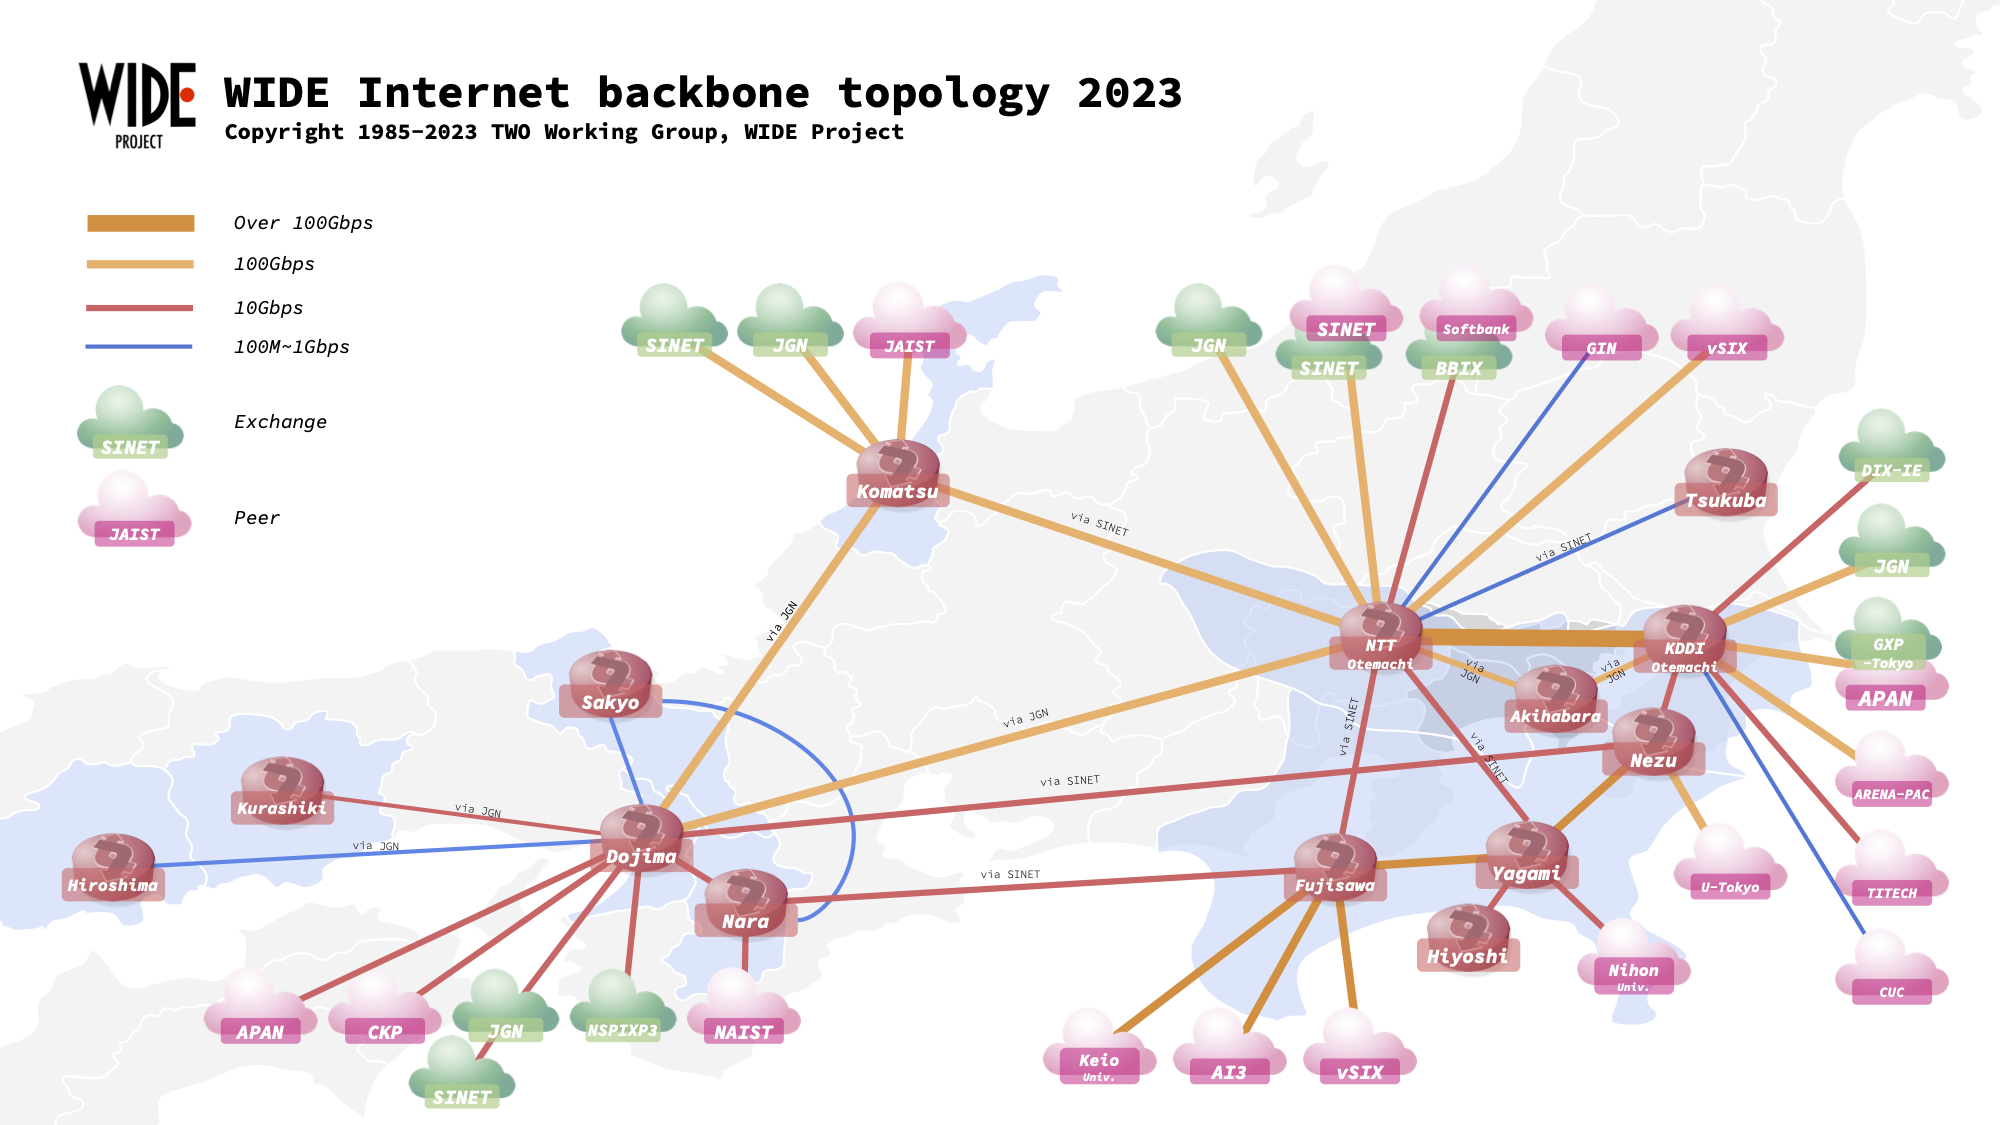
\includegraphics[width=\linewidth]{MAWI/wide topology.png}
    \caption{MAWI: WIDE Internet backbone topology 2023}
    \label{MAWI: WIDE Internet backbone topology 2023}
\end{figure}

\subsection{MAWI} The Measurement and Analysis on the WIDE (AS2500) Internet (MAWI) Working Group is a collaborative effort by multiple network research and academic institutions based in Japan \cite{271335}. Its primary objective is to provide invaluable insights into the backbone infrastructure of Japan through network research. A topology map of the WIDE network is shown in Figure \ref{MAWI: WIDE Internet backbone topology 2023}.

MAWI is one of the most reputable Internet weather maps and statistics sources, with its traffic archive serving as the basis of network research for several years. This archive has been in operation since 1999, except for a few minor interruptions. As a result, exhaustive research methodologies, including longitudinal studies, are applied.

The set of tools and the data repository are open source, making them accessible to anyone interested in network research \cite{MAWIDataset}. Packet traces are collected using the network traffic monitoring software tcpdump \cite{tcpdump} and anonymized with a modified version of tcpdriv \cite{TCPDPRIV}. Network tracing starts every day from 14:00 to 14:15 Japanese Standard Time, with packet traces collected and made public on the data repository platform. The traces are highly aggregated, with each 15-minute trace containing approximately 300k-500k unique IP addresses \cite{5061979}.

The MAWI Working Group has several sample points from the WIDE backbone infrastructure, with sample point \textbf{B} and sample point \textbf{F} being the largest datasets. The sample point \textbf{B} was collected between January 2001 and June 2006, while the sample point \textbf{F} data was collected from October 2006 onwards. Sample point \textbf{F} monitors a 1Gb/s transport link from Tokyo to the NTT Global IP Network (AS2914). Traffic on the link was port mirrored to a 10Gb/s link on the router and captured using a commodity PC server and a 10GbE NIC running FreeBSD. Different sample points originate due to different settings and newer or older links.

An example trace from the sample point \textbf{F} was taken on December 10, 2023, and is to be analyzed in the following \cite{traceMAWI}:

\begin{figure}
        \centering
        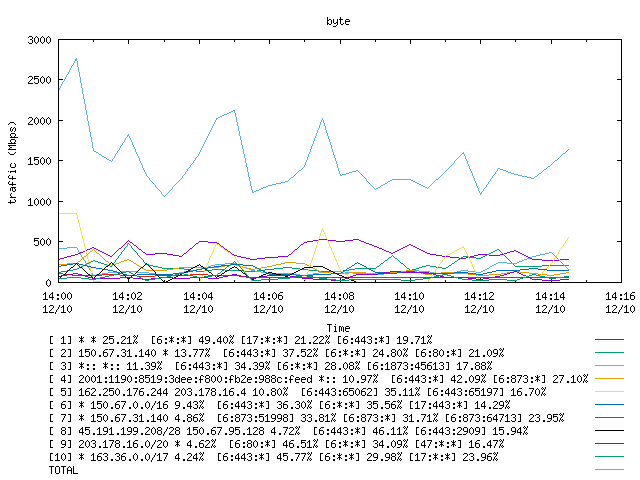
\includegraphics[width=1\linewidth]{MAWI/MAWI 2023-12-10 aggregated analysis byte.png}
        \caption{MAWI: Aggregated flow of traffic}
        \label{MAWI: Aggregated Flow Byte}
\end{figure}

Figure \ref{MAWI: Aggregated Flow Byte} provides a comprehensive summary of the aggregated flow of traffic on the WIDE Internet. Figure \ref{MAWI: Aggregated Flow Byte} offers a graphical representation of the traffic stream in Mb/s over time. It ranks several connections below the graph, based on their percentages of total traffic. The graph illustrates changes in the traffic stream over time.

For example, the second-ranked connection in Figure \ref{MAWI: Aggregated Flow Byte} uses the IPv4 protocol and originates from the source address 150.67.31.140. The destination address is specified as the wildcard character "*" which in this case represents 0.0.0.0/0 for IPv4. This connection had a total usage of 13.77\%. The connection also has statistical information on the protocols and ports used and their percentages of traffic on that connection. 

To further elaborate, the connection had 37.52\% of traffic using the Internet protocol TCP (Transmission Control Protocol). This value is based on Assigned Internet Protocol Numbers and was used on HTTPS (Hypertext Transfer Protocol Secure). The destination port specified for this connection is the wildcard "*", which stands for any port in the destination. This information is crucial to analyze and understand the network traffic flow and usage patterns at the WIDE Internet.

The plot graphs and the underlying statistics were made by Agurim, a traffic monitoring system developed within the WIDE project to analyze out- and ongoing traffic traces. It utilizes multidimensional flow aggregation, which easily captures dynamic changes in traffic \cite{179442}. 

Figure \ref{MAWI: Aggregated Flow Byte} provides substantial information on how traffic changes over time, especially when combined with other traffic traces. Case studies can be made possible at individual times through specific days, and attacks and anomalies can be identified faster and more efficiently using the collected traces.

The MAWI data repository is a public repository that provides real public data, which can be accessed and used freely by researchers for various purposes. However, since data sets contain sensitive user information, it is important to ensure that users' privacy is protected. To this end, the MAWI Working Group has established guidelines for privacy protection, which must be followed by users of data sets \cite{MAWIGuideline}. 

According to the MAWI guideline, the first step in anonymizing traffic traces is to remove any payload that the TCP and UDP protocols may contain. This is because the payload can contain sensitive user information, such as passwords or credit card numbers. If there are packets with another protocol on top and the inner packet header does not contain any private user information, then the inner packet header is left intact.

The second step is to scramble the source and destination addresses of the packets, which is done based on two methods. The first method involves mapping an IP address to a different IP address using a hash function. This ensures that the original IP address cannot be traced back to the user. The second method is used if two IP addresses have a common address prefix. In this case, both IP addresses are assigned to addresses with a common address prefix of the same length. Addresses that lack user identifiers, such as broadcast, multicast, and private addresses, are not scrambled.

When operating in IPv6 mode, link-local addresses, and site-local addresses are also scrambled. This is because these addresses may contain user MAC addresses, which can be used to identify users. Ethernet headers, on the other hand, do not have to be scrambled, since they are internal nodes' or backbone networks' addresses. 

By following these guidelines, data sets from the MAWI data repository can be used for research purposes without violating the privacy of users.

The MAWI Working Group suggests in the guideline three different scrambling policies for consistency, where the guideline recommends the second option:
\begin{itemize}
    \item A TCP session in a single data set is mapped to the same address. 
    \item All occurrences of addresses in a data set are scrambled to a single address.
    \item All occurrences of addresses in several data sets are scrambled to a single address.
\end{itemize}

Following the guidelines set by the WIDE project, the privacy of the end-users is guaranteed, and the risk of revealing sensitive information is kept to a minimum. This ensures that the MAWI dataset can be used for research purposes without compromising user confidentiality.

The MAWI archive has been a valuable resource for network researchers, with several real-world applications emerging from it. One such project is the MAWILab database, which helps researchers evaluate traffic anomaly detection methods. The database includes both sample points \textbf{B} and \textbf{F} mentioned earlier, and it is updated daily with new traffic traces and possible anomalies  \cite{mawilab}. 

The MAWILab project is an excellent resource for researchers looking to study anomaly detection in real-world traffic scenarios. By using the MAWI dataset, they can gain valuable insights into network behavior and develop effective methods for identifying and mitigating anomalies. With the database being updated daily, researchers can stay up-to-date with the latest traffic patterns and anomalies, making it a valuable tool for ongoing research.

\begin{figure}
        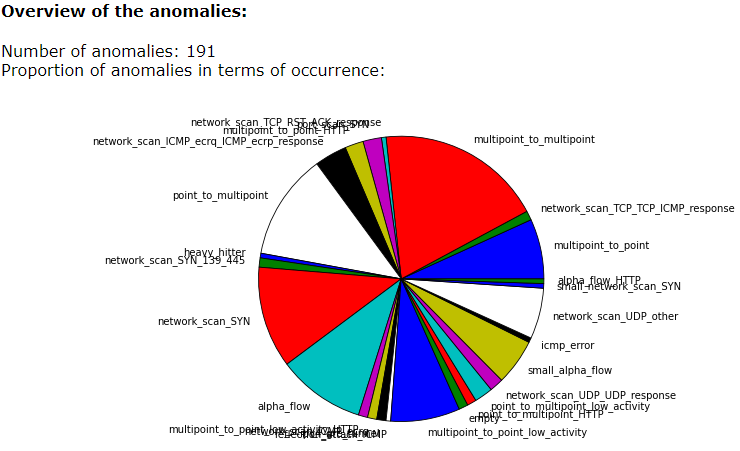
\includegraphics[width=\linewidth]{MAWI/MAWILab.PNG}
        \caption{MAWI: MAWILab Anomaly Detection Overview}
        \label{MAWI: MAWILab Anomaly Detection Overview}
\end{figure}

In Figure \ref{MAWI: MAWILab Anomaly Detection Overview}, MAWILab provides anomaly detection analysis for a specific trace on August 2, 2023, from the MAWI archive\footnote{\url{http://www.fukuda-lab.org/mawilab/v1.1/2023/08/02/20230802.html}}. It detected 191 anomalies, of which several were network scans or multipoint-to-multipoint connections. MAWILab also provides a detailed table of all anomalies, with attributes like source or destination IP address, source or destination port, and what type of taxonomy was used, as shown in \ref{anomaly} (some columns were removed for better visibility, for example, source port, destination IP address, and so on).

\begin{table}[!ht]
    \centering
    \caption{MAWI: Anomalies in trace of August 2, 2023}
    \label{anomaly}
    \begin{tabular}{|l|l|l|l|l|l|l|}
    \hline
        anomalyID &  srcIP & dstPort & nbDetectors \\ \hline
        109 & 185.233.188.247 & 22 & anomalous \\ \hline
        110 & 183.112.233.74 & 22 & anomalous \\ \hline
        113 & 119.160.59.14 & 6379 & anomalous \\ \hline
        114 & 81.73.84.186 & 6379 & anomalous \\ \hline
        116 & 188.93.176.191 & 2048 & anomalous \\ \hline
        116 & 188.93.176.191 & 49152 & anomalous \\ \hline
    \end{tabular}
\end{table}

The MAWI Working Group has facilitated two significant longitudinal analyses, thanks to its exceptional preservation, archiving, and frequent updating of datasets. Longitudinal analyses focus on studying observations made over an extended period to assess changes and developments in underlying structures, thus paving the way for understanding long-term trends and patterns.

The first longitudinal analysis conducted was a comprehensive seven-year study that revealed significant day-to-day variability, which was influenced by congestion and random anomalies. This variability made it impossible to draw conclusive remarks about the long-term evolution of network traffic. However, the authors of the study were able to develop methodological approaches to prevent day-to-day incidental variability using sketches and median averages. This improved the reliability of traffic estimation and focused on the long-term evolution. Additionally, the study showed that Internet traffic remained stable over the entire period \cite{5061979}.

The second longitudinal analysis was conducted 14 years after the founding of the MAWI Working Group. The 14-year longitudinal study on the MAWI dataset traffic highlighted two main scaling ranges in Internet traffic, coarse and fine scales. These scaling ranges referred to smaller and bigger versions of traffic. This indicates a consistent biscaling system across time, despite technological evolution. At coarse scales, long-range dependence (LRD) accurately represented traffic dynamics. In contrast, on fine scales, multifractal properties were more descriptive, contributing to the temporal burstiness observed in Internet traffic \cite{7878657}.

\begin{figure}
    \centering
    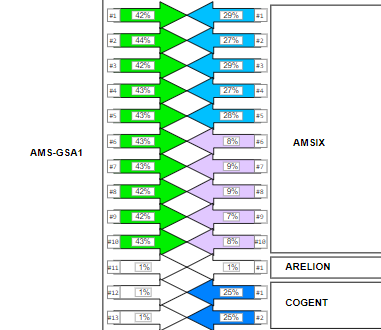
\includegraphics[width=\linewidth]{OVH/ovh.png}
    \caption{OVH: Excerpt from the European backbone network}
    \label{OVH: Excerpt from the European backbone network}
\end{figure}

Overall, it is evident that the MAWI Working Group has greatly helped the networking community by providing helpful tools such as agurim and tcpdpriv, as well as the data repository itself for research purposes. The data sets have laid a good structure by delivering continuous traces and anonymizing them in the process. These insights have provided a better understanding of the behavior of Internet traffic over an extended period, paving the way for more effective network management and infrastructure improvements.

\subsection{OVH}
OVH is a cloud computing company headquartered in France. It offers a wide array of web services, including virtual private or dedicated servers. With over 20 years of industry experience, OVH has become one of the largest hosting providers worldwide. It currently operates more than 40 data centers in nine countries, providing reliable and secure hosting solutions to millions of users around the world \cite{ovhcloudwebsite}.

The OVH cloud provider has created an Internet weather map that provides valuable information regarding its data centers, peers, and link loads between them \cite{ovhcloud}. This map is an essential tool for network administrators and users to monitor and analyze the performance of OVH's infrastructure. Figure \ref{OVH: Excerpt from the European backbone network} of the map illustrates the Global Switch and Digital Realty data centers in Amsterdam as a large rectangle while peers are represented as smaller rectangles. The links, which reflect the out- and ongoing bandwidth, are displayed as arrows that emanate from the respective rectangle. 

The arrows are color-coded according to the bandwidth loads, which follow the criteria shown in Figure \ref{OVH: Links bandwidth load scale}. For example, the Amsterdam Internet Exchange has ten parallel links connected to the Global Switch data center. The first five links exhibit an outgoing bandwidth load ranging from 27\% to 29\%, while the other five have an outgoing bandwidth load ranging from 7\% to 9\%. This indicates that the latter links serve as backup outgoing links to ensure redundancy. In contrast, all ongoing bandwidth loads have similar percentages ranging from 42\% to 44\%, distributing the workload equally among all ongoing links. 

The OVH Internet weather map provides a comprehensive view of OVH's data center performance, peers, and link loads. It facilitates effective network management and helps ensure optimal performance, reliability, and availability of OVH's infrastructure.

\begin{figure}
    \centering
    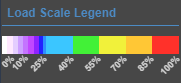
\includegraphics{OVH/scale.png}
    \caption{OVH: Links bandwidth load scale}
    \label{OVH: Links bandwidth load scale}
\end{figure}

The OVH Internet weather map has been instrumental in the development of SCMon, which is a monitoring technique that employs Segment Routing to send probes over cycles. This innovative technique encodes the routing path directly into the packet header using a well-ordered list of segments, thereby enhancing the way data packets are routed through a network. The publicly available topology of OVH was used to evaluate the effectiveness of SCMon, and the experiments revealed favorable results. Even with a limited number of cycles, the location of failures could be accurately identified in milliseconds \cite{7524410}.

In another study, the importance of rate adaptation was analyzed on daily timescales by studying the OVH Internet weather map. It was revealed that the utilization of the OVH network was low and predictable, while parallelism was utilized significantly, resulting in a reduction in utilization. This led to the creation of redundant links that could be turned off to save energy. Furthermore, it was discovered that downgrading the links on the OVH network from 100GbE to 10GbE or 25GbE was more energy efficient \cite{10.1145/3604930.3605713}.

\subsection{MANDA}
The Metropolitan Area Network Darmstadt (MANDA) is a regional high-speed network that connects numerous scientific institutions situated in the vicinity of the city of Darmstadt in Germany. The primary objective of MANDA is to enable seamless collaboration among the various institutions and offer opportunities to share resources and knowledge. Through the shared usage of the network, energy conservation is promoted, making MANDA a valuable asset in promoting sustainable practices \cite{manda1}. The MANDA project is efficiently coordinated by the Hochschulrechenzentrum, while day-to-day operations are managed by man-da.de GmbH \cite{manda2}. 

The network's topology, partly shown in Figure \ref{MANDA: MANDA Network Weathermap} provides a detailed view of the interconnections between nodes in the city of Darmstadt. Each node represents a specific landmark or place in the city, forming a complex web of connections that allows for seamless communication and resource sharing. At the moment, the MANDA weather map and statistics are not accessible to the general public. Access to this website and its valuable information is restricted and requires special credentials. However, for those interested in obtaining historical data, the Wayback Machine offers a collection of snapshots of some subpages from the past. These snapshots may provide useful insight into past weather patterns and trends \cite{gartner}.

\begin{figure}
    \centering
    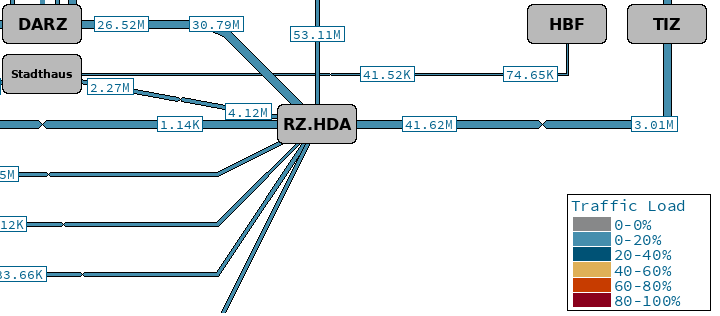
\includegraphics[width=\linewidth]{MANDA/manda.png}
    \caption{MANDA: Excerpt from the MANDA Network Weathermap and load scale}
    \label{MANDA: MANDA Network Weathermap}
\end{figure}

In the network diagram displayed in Figure \ref{MANDA: MANDA Network Weathermap}, the connection or link between two nodes can be seen as a colored line. These lines are labeled with the outgoing and ongoing bandwidth to provide information about the amount of data that is being transmitted. The color of each line is based on the traffic load percentage scale, which indicates the level of activity on that particular link. 

As an example, the node RZ.HDA, which stands for Rechenzentrum Hochschule Darmstadt. From the perspective of the snapshot in Figure \ref{MANDA: MANDA Network Weathermap}, we can see that this node has a connection with DARZ, Darmstadt Rechenzentrum. The outgoing traffic bandwidth for RZ.HDA is 30.79Mb/s, which means that data is being transmitted from this node to DARZ at this rate. Meanwhile, an ongoing traffic bandwidth of 26.52Mb/s is being received by RZ.HDA, indicating that data is being received from DARZ at this rate. The color-coded lines in the network diagram provide useful information about the traffic load on each link, while the bandwidth labels give us a more detailed understanding of the amount of data being transmitted in each direction.

\begin{figure}
    \centering
    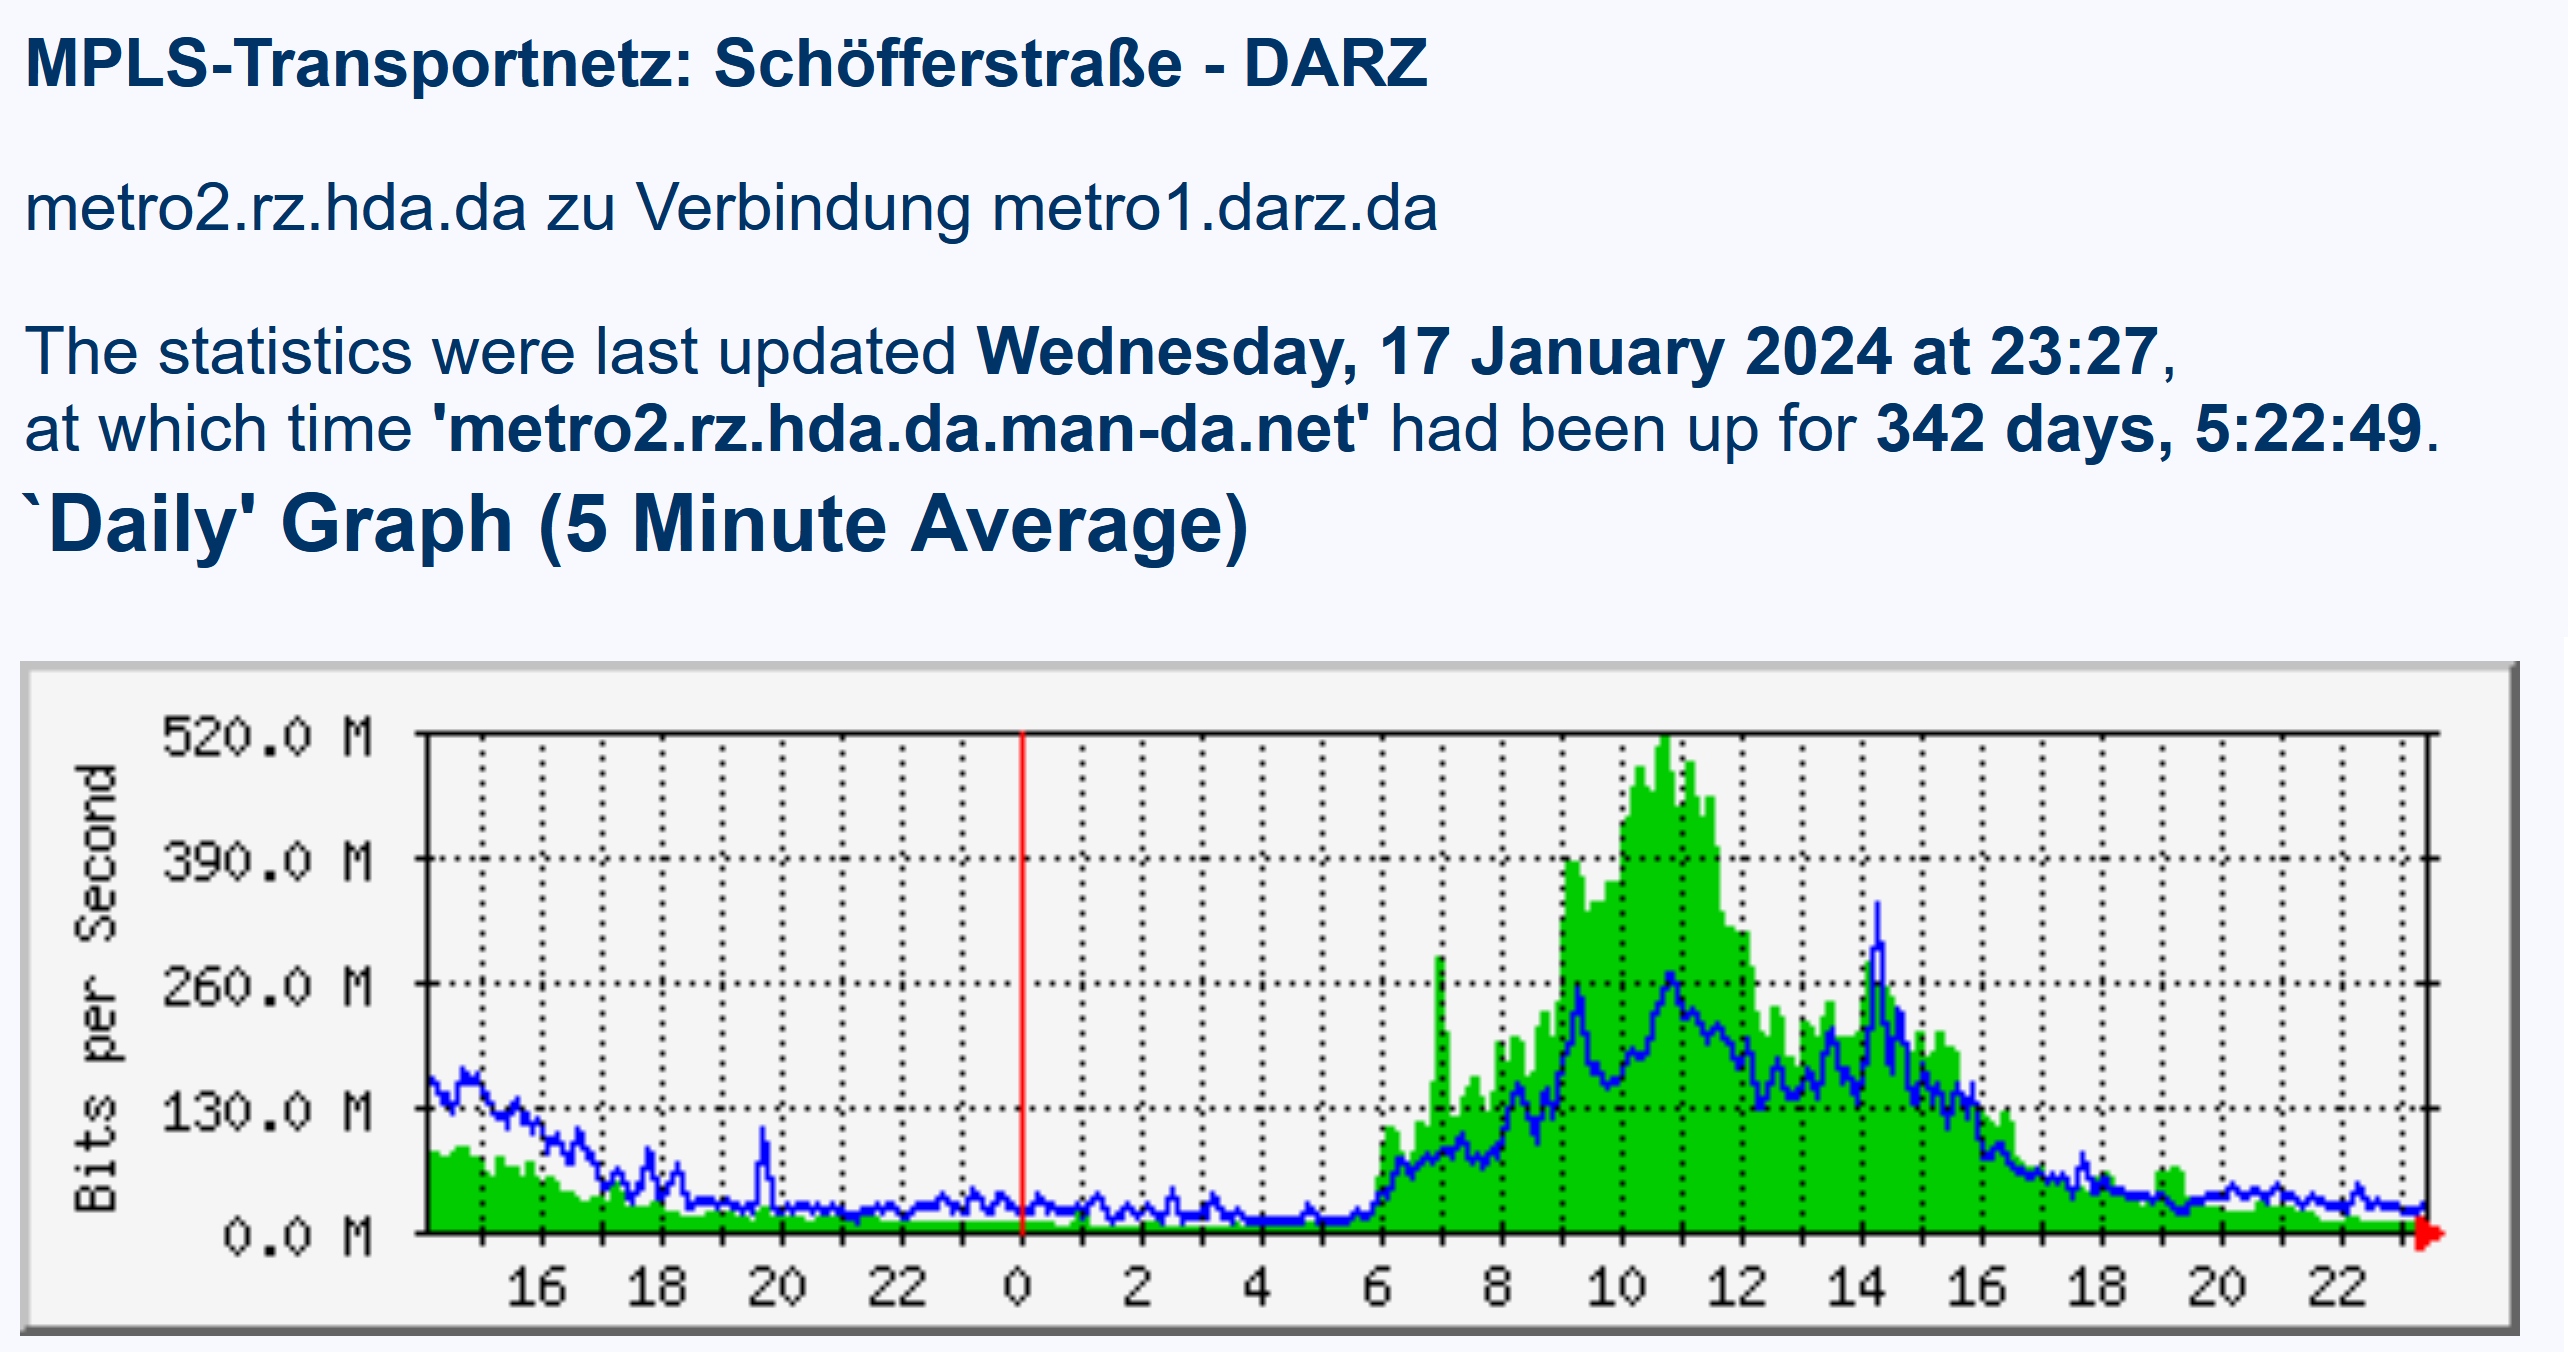
\includegraphics[width=\linewidth]{MANDA/statistics link darmsdat.PNG}
    \caption{MANDA: Daily statistics for the link between RZ.HDA and DARZ}
    \label{MANDA: Daily statistics of}
\end{figure}

\begin{table}[!ht]
    \centering
    \caption{MANDA: Recorded bandwidth for the link between RZ.HDA and DARZ}
    \label{MANDA: Recorded bandwidth for the link between RZ.HDA and DARZ}
    \begin{tabular}{|l|l|l|l|}
    \hline
        & Max                & Average           & Current             \\ \hline
    In  & 511.7 Mb/s (5.1\%) & 90.1 Mb/s (0.9\%) & 8217.6 Kb/s (0.1\%) \\ \hline
    Out & 334.6 Mb/s (3.3\%) & 72.3 Mb/s (0.7\%) & 17.4 Mb/s (0.2\%) \\ \hline
    \end{tabular}
\end{table}

The statistics webpage is an informative platform that provides daily, weekly, and yearly monthly statistics for various links. By clicking on a link, the user can access the webpage and view the statistics for that particular link—the link between RZ.HDA and DARZ, for instance, had their daily statistics shown in Figure \ref{MANDA: Daily statistics of}. The webpage displays the name and category of the link, which provides useful information about the link's location and function. For example, the link "MPLS-Transportnetz: Schöfferstraße - DARZ" in Figure \ref{MANDA: Daily statistics of} represents the connection between Hochschule Darmstadt and DARZ. Schöfferstraße is the street where Hochschule Darmstadt is located, and its node name is labeled as "metro2.rz.hda.da". Meanwhile, DARZ's node is labeled as "metro1.darz.da". 

Additionally, the statistics for each link are updated every 5 to 10 minutes, ensuring that the data provided is accurate and up-to-date. The webpage also displays the uptime of each link, as seen in Figure \ref{MANDA: Daily statistics of}, where the link "metro2.rz.hda.da.man-da.net" has been up for 342 days and approximately 5 hours. 

The daily graph for each link is shown in Figure \ref{MANDA: Daily statistics of}, and weekly and monthly graphs are available as well. The graph represents the stream of traffic in bits per second over time for a particular day (and a few hours). Moreover, the webpage records and displays maximal, average, and current statistics for both outgoing and ongoing bandwidth, providing a comprehensive overview of the link's performance, as shown in Table \ref{MANDA: Recorded bandwidth for the link between RZ.HDA and DARZ}. 

Furthermore, the webpage maintains a detailed history of all data volumes and average traffic bandwidths going through TU Darmstadt from 2004 onwards. The data for December 2023 is shown in Figure \ref{MANDA: Data volumes of TU Darmstadt}, and users can select a particular month to view the data volumes and average traffic bandwidth. Overall, the statistics webpage is a valuable resource that provides users with detailed and up-to-date information about the performance of various links.

One issue with the MANDA network is that it doesn't maintain an archive of its statistics. This poses a challenge for research institutions looking to study the network and its data. Without archived data, researchers would be unable to conduct in-depth analyses and draw conclusions about traffic patterns under specific conditions such as changes in weather, political and social movements, and other related factors. However, with the help of archiving software, researchers can retrieve and store data for future reference and analysis. By analyzing the data in detail, researchers can gain a better understanding of the underlying causes and effects of various factors that affect traffic patterns, which can help in developing more effective strategies and solutions to manage traffic and improve overall traffic flow.

\begin{figure}
    \centering
    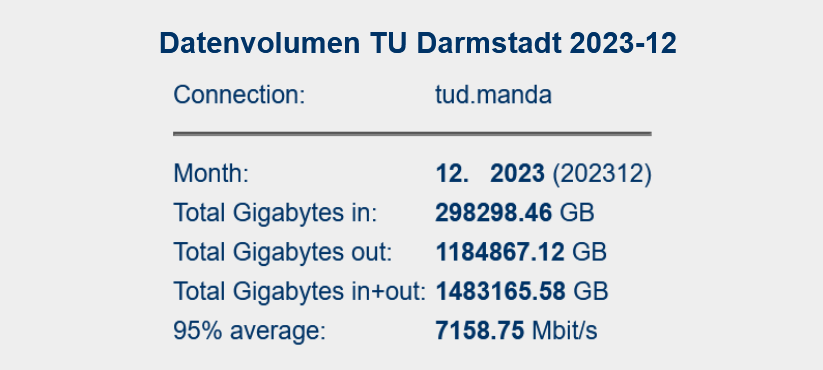
\includegraphics[width=\linewidth]{MANDA/pastedImage.png}
    \caption{MANDA: Data volumes of TU Darmstadt}
    \label{MANDA: Data volumes of TU Darmstadt}
\end{figure}

\subsection{SWITCH}

The Switch Foundation is a private, non-profit organization that was established in 1987 in collaboration with the Swiss Confederation and eight university cantons. The foundation is primarily focused on the maintenance, development, and enhancement of a highly interconnected infrastructure for research and education purposes in Switzerland. The foundation aims to provide seamless and secure digital communication services to the Swiss academic and research community. It also strives to facilitate the growth and expansion of research and education networks in the country, which can be utilized by a broad range of institutions and organizations \cite{switch}.

\begin{figure}
    \centering
    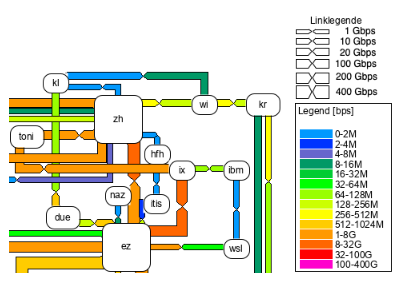
\includegraphics[width=\linewidth]{SWITCH/switch.PNG}
    \caption{Switch: Excerpt from the national SWITCH Internet Weather Map}
    \label{SWITCH: National SWITCH Internet Weather Map}
\end{figure}

The Switch Foundation showcases two Internet weather maps, national \cite{switchnational} and international \cite{switchinternational}. The national Internet weather map is depicted in Figure \ref{SWITCH: National SWITCH Internet Weather Map} as a graph representation with nodes being research institutions or universities and vertices being the links between each institution. Link capacity (width) and usage (color) are also shown in Figure \ref{SWITCH: National SWITCH Internet Weather Map}. When hovering over a certain link, additional statistics will show for that link. For example, the link between "ez" (Eidgenössische Technische Hochschule Zürich) and "ix" (Equinix) gives the statistics shown in Figure \ref{SWITCH: Daily statistics between ETHZ and Equinix}. The international Internet weather map is analogously defined.

One of the other services offered by Switch Foundation is the hosting of traffic graphs for international links to institutions such as GÉANT, Lumen, Cogent, and many others \cite{switchgraph}. These traffic graphs contain daily, weekly, monthly, and yearly statistics, which can be useful for analyzing network performance and identifying any potential issues. Moreover, Switch Foundation maintains detailed records of data volumes for each month, providing valuable insights into the overall network usage patterns. For instance, in December 2023, the network experienced a total data volume of 27321 TB, which is a significant amount. Further information can be accessed by using access from one of the involved institutions in the Switch Foundation network.

Overall, the services provided by the Switch Foundation can be utilized to research Swiss network traffic data by storing publicly available information and analyzing it to conclude network behavior.

\begin{figure}
    \centering
    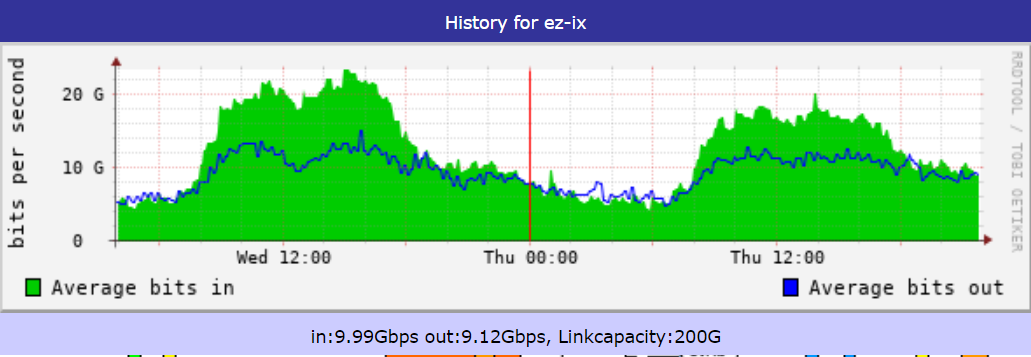
\includegraphics[width=\linewidth]{SWITCH/stats ez-ix.PNG}
    \caption{Switch: Daily statistics for the link between ETHZ and Equinix}
    \label{SWITCH: Daily statistics between ETHZ and Equinix}
\end{figure}

\section{Conclusion}

The paper emphasizes the crucial role played by Internet weather maps and statistics in the field of data networking. These maps serve as a valuable resource for network administrators and engineers to monitor and evaluate network performance, and ensure its security and reliability. They provide a real-time view of network activity, such as traffic volume, latency, and packet loss, helping to identify potential issues and troubleshoot them proactively. 

Moreover, this paper provides a detailed analysis of several Internet weather maps that can aid in further research on network behavior. By examining these maps, researchers can gain insights into the underlying factors that impact network performance, such as congestion, routing, and network topology. This information can be used to optimize network design and management, enhance the quality of service, and improve the overall user experience.

\bibliographystyle{ACM-Reference-Format}
\bibliography{bibliography}

\appendix

\section{Honorable Mentions}
In the following section, I will mention several Internet weather maps that hold interesting information but could not be described in the paper.
\subsection{i2basque}
i2basque is a telecommunications and information and communication technology (ICT) service provider that was established in 2005 as part of the "Plan Euskadi en la Sociedad de la Información" program developed by the Basque Government's Department of Education. Its primary objective is to provide ICT infrastructure services to universities, scientific facilities, hospitals, and other institutions in the region \cite{i2basque}.
\subsection{REANNZ}
The Research and Education Advanced Network New Zealand (REANNZ) network was launched in 2007 to provide an infrastructure for members to collaborate and contribute to science and research initiatives in New Zealand and across the globe. The network is the backbone of New Zealand's research and education sector \cite{REANNZ}.
\subsection{TWAREN}
The TaiWan Advanced Research and Education Network (TWAREN) is an alliance of universities and government and research institutions in Taiwan. It provides a 100GbE backbone infrastructure with a fault-tolerant network architecture. Furthermore, TWAREN provides 30Gb/s bandwidth in total to major networks in world continents, such as America, Europe, and Asia \cite{TWAREN}.
\subsection{RUB}
The Ruhr University Bochum is a public research university in Bochum, Germany. The Internet weather map of RUB has a complex structure with over 50 nodes, encompassing traffic statistics to all relevant landmarks in the city \cite{rub}.
\subsection{Uninett}
Uninett is a state-owned company that operates the national research and education network of Norway. The network connects the neighboring countries with Norway, such as Sweden, Finland, and St. Petersburg \cite{Uninett}.
\subsection{CSNET}
The Czech Education and Scientific NETwork (CESNET) was established by Czech public universities and the Academy of Sciences of the Czech Republic. It is the developer and operator of the technological infrastructure for science, research, and education in the Czech Republic. As part of its responsibilities, it researches advanced network technologies that originate from hybrid networking and programmable hardware \cite{CESNET}.

For further research, the following Internet weather maps can also be analyzed: 
\begin{itemize}
    \item MERLIN \cite{merlin}
    \item INEX \cite{inex}
    \item IPTP \cite{iptp}
    \item BCNET \cite{Bcnet}
\end{itemize}
\section{Tools}
The following section will refer to tools that were used to represent the Internet weather maps and statistics.
\subsection{PHP Weathermap}

PHP Weathermap is a highly useful and efficient open-source network visualization tool that enables users to create an overview of network activity in a map format. The tool works by collecting data from several programs, such as SNMP or MRTG as in  \ref{MRTG}, which can then be used to create detailed network maps. 

One of the major benefits of PHP Weathermap is its comprehensive and detailed documentation, which makes it easy for users to understand and use the tool effectively. Additionally, PHP Weathermap comes equipped with an interactive editor that simplifies the process of creating network maps. 

PHP Weathermap is a popular choice among many ISPs, Internet exchanges, academic institutions, and other organizations. It was developed primarily in the PHP programming language, with JavaScript being the secondary language. Most of the Internet weather maps that you might have come across have used PHP Weathermap to represent their network map. 

Overall, PHP Weathermap is a valuable tool that provides users with a clear and concise overview of their network activity and has proven to be a reliable and widely used resource in the industry.

\subsection{MRTG}\label{MRTG}
The Multi Router Traffic Grapher (MRTG) is a powerful tool utilized to monitor the traffic load on network links. It is capable of generating HTML pages that contain PNG images and statistics, giving users detailed insights into their network performance. Figure \ref{MANDA: Daily statistics of} provides a snapshot of the kind of information MRTG can provide. 

MRTG operates by using SNMP queries at regular intervals to generate graphs that display network traffic trends. In addition to monitoring network traffic, MRTG can also be used to measure other critical performance metrics, such as CPU load, disk availability, temperature, and much more. 

This tool has been extensively used in the MANDA and Switch environments, where it has proven to be a reliable and informative solution for network monitoring and performance analysis. With its ability to collect and analyze data from multiple sources, MRTG is a valuable asset for any organization seeking to optimize its network performance.

\end{document}